% Created by tikzDevice version 0.10.1 on 2018-01-22 11:53:28
% !TEX encoding = UTF-8 Unicode
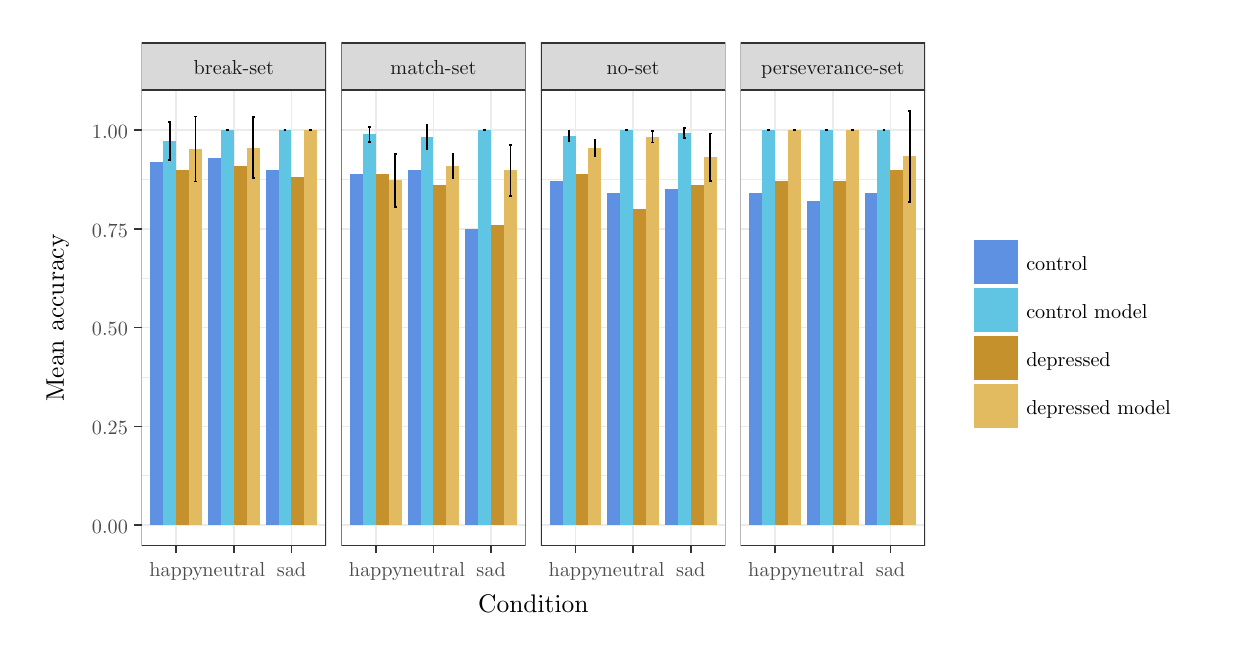
\begin{tikzpicture}[x=1pt,y=1pt]
\definecolor{fillColor}{RGB}{255,255,255}
\path[use as bounding box,fill=fillColor,fill opacity=0.00] (0,0) rectangle (433.62,216.81);
\begin{scope}
\path[clip] (  0.00,  0.00) rectangle (433.62,216.81);
\definecolor{drawColor}{RGB}{255,255,255}
\definecolor{fillColor}{RGB}{255,255,255}

\path[draw=drawColor,line width= 0.6pt,line join=round,line cap=round,fill=fillColor] (  0.00,  0.00) rectangle (433.62,216.81);
\end{scope}
\begin{scope}
\path[clip] ( 41.17, 29.59) rectangle (107.82,194.25);
\definecolor{fillColor}{RGB}{255,255,255}

\path[fill=fillColor] ( 41.17, 29.59) rectangle (107.82,194.25);
\definecolor{drawColor}{gray}{0.92}

\path[draw=drawColor,line width= 0.3pt,line join=round] ( 41.17, 54.91) --
	(107.82, 54.91);

\path[draw=drawColor,line width= 0.3pt,line join=round] ( 41.17, 90.59) --
	(107.82, 90.59);

\path[draw=drawColor,line width= 0.3pt,line join=round] ( 41.17,126.28) --
	(107.82,126.28);

\path[draw=drawColor,line width= 0.3pt,line join=round] ( 41.17,161.96) --
	(107.82,161.96);

\path[draw=drawColor,line width= 0.6pt,line join=round] ( 41.17, 37.07) --
	(107.82, 37.07);

\path[draw=drawColor,line width= 0.6pt,line join=round] ( 41.17, 72.75) --
	(107.82, 72.75);

\path[draw=drawColor,line width= 0.6pt,line join=round] ( 41.17,108.44) --
	(107.82,108.44);

\path[draw=drawColor,line width= 0.6pt,line join=round] ( 41.17,144.12) --
	(107.82,144.12);

\path[draw=drawColor,line width= 0.6pt,line join=round] ( 41.17,179.80) --
	(107.82,179.80);

\path[draw=drawColor,line width= 0.6pt,line join=round] ( 53.67, 29.59) --
	( 53.67,194.25);

\path[draw=drawColor,line width= 0.6pt,line join=round] ( 74.50, 29.59) --
	( 74.50,194.25);

\path[draw=drawColor,line width= 0.6pt,line join=round] ( 95.32, 29.59) --
	( 95.32,194.25);
\definecolor{fillColor}{RGB}{226,186,95}

\path[fill=fillColor] ( 58.36, 37.07) rectangle ( 63.04,173.00);
\definecolor{fillColor}{RGB}{196,145,45}

\path[fill=fillColor] ( 53.67, 37.07) rectangle ( 58.36,165.53);
\definecolor{fillColor}{RGB}{95,197,226}

\path[fill=fillColor] ( 48.98, 37.07) rectangle ( 53.67,175.83);
\definecolor{fillColor}{RGB}{95,145,226}

\path[fill=fillColor] ( 44.30, 37.07) rectangle ( 48.98,168.38);
\definecolor{fillColor}{RGB}{226,186,95}

\path[fill=fillColor] ( 79.18, 37.07) rectangle ( 83.87,173.46);
\definecolor{fillColor}{RGB}{196,145,45}

\path[fill=fillColor] ( 74.50, 37.07) rectangle ( 79.18,166.95);
\definecolor{fillColor}{RGB}{95,197,226}

\path[fill=fillColor] ( 69.81, 37.07) rectangle ( 74.50,179.80);
\definecolor{fillColor}{RGB}{95,145,226}

\path[fill=fillColor] ( 65.12, 37.07) rectangle ( 69.81,169.81);
\definecolor{fillColor}{RGB}{226,186,95}

\path[fill=fillColor] (100.01, 37.07) rectangle (104.69,179.80);
\definecolor{fillColor}{RGB}{196,145,45}

\path[fill=fillColor] ( 95.32, 37.07) rectangle (100.01,162.67);
\definecolor{fillColor}{RGB}{95,197,226}

\path[fill=fillColor] ( 90.64, 37.07) rectangle ( 95.32,179.80);
\definecolor{fillColor}{RGB}{95,145,226}

\path[fill=fillColor] ( 85.95, 37.07) rectangle ( 90.64,165.53);
\definecolor{drawColor}{RGB}{0,0,0}

\path[draw=drawColor,line width= 0.6pt,line join=round] ( 60.18,184.77) --
	( 61.22,184.77);

\path[draw=drawColor,line width= 0.6pt,line join=round] ( 60.70,184.77) --
	( 60.70,161.23);

\path[draw=drawColor,line width= 0.6pt,line join=round] ( 60.18,161.23) --
	( 61.22,161.23);

\path[draw=drawColor,line width= 0.6pt,line join=round] ( 50.81,182.70) --
	( 51.85,182.70);

\path[draw=drawColor,line width= 0.6pt,line join=round] ( 51.33,182.70) --
	( 51.33,168.97);

\path[draw=drawColor,line width= 0.6pt,line join=round] ( 50.81,168.97) --
	( 51.85,168.97);

\path[draw=drawColor,line width= 0.6pt,line join=round] ( 81.00,184.44) --
	( 82.05,184.44);

\path[draw=drawColor,line width= 0.6pt,line join=round] ( 81.52,184.44) --
	( 81.52,162.47);

\path[draw=drawColor,line width= 0.6pt,line join=round] ( 81.00,162.47) --
	( 82.05,162.47);

\path[draw=drawColor,line width= 0.6pt,line join=round] ( 71.63,179.80) --
	( 72.67,179.80);

\path[draw=drawColor,line width= 0.6pt,line join=round] ( 72.15,179.80) --
	( 72.15,179.80);

\path[draw=drawColor,line width= 0.6pt,line join=round] ( 71.63,179.80) --
	( 72.67,179.80);

\path[draw=drawColor,line width= 0.6pt,line join=round] (101.83,179.80) --
	(102.87,179.80);

\path[draw=drawColor,line width= 0.6pt,line join=round] (102.35,179.80) --
	(102.35,179.80);

\path[draw=drawColor,line width= 0.6pt,line join=round] (101.83,179.80) --
	(102.87,179.80);

\path[draw=drawColor,line width= 0.6pt,line join=round] ( 92.46,179.80) --
	( 93.50,179.80);

\path[draw=drawColor,line width= 0.6pt,line join=round] ( 92.98,179.80) --
	( 92.98,179.80);

\path[draw=drawColor,line width= 0.6pt,line join=round] ( 92.46,179.80) --
	( 93.50,179.80);
\definecolor{drawColor}{gray}{0.20}

\path[draw=drawColor,line width= 0.6pt,line join=round,line cap=round] ( 41.17, 29.59) rectangle (107.82,194.25);
\end{scope}
\begin{scope}
\path[clip] (113.32, 29.59) rectangle (179.96,194.25);
\definecolor{fillColor}{RGB}{255,255,255}

\path[fill=fillColor] (113.32, 29.59) rectangle (179.96,194.25);
\definecolor{drawColor}{gray}{0.92}

\path[draw=drawColor,line width= 0.3pt,line join=round] (113.32, 54.91) --
	(179.96, 54.91);

\path[draw=drawColor,line width= 0.3pt,line join=round] (113.32, 90.59) --
	(179.96, 90.59);

\path[draw=drawColor,line width= 0.3pt,line join=round] (113.32,126.28) --
	(179.96,126.28);

\path[draw=drawColor,line width= 0.3pt,line join=round] (113.32,161.96) --
	(179.96,161.96);

\path[draw=drawColor,line width= 0.6pt,line join=round] (113.32, 37.07) --
	(179.96, 37.07);

\path[draw=drawColor,line width= 0.6pt,line join=round] (113.32, 72.75) --
	(179.96, 72.75);

\path[draw=drawColor,line width= 0.6pt,line join=round] (113.32,108.44) --
	(179.96,108.44);

\path[draw=drawColor,line width= 0.6pt,line join=round] (113.32,144.12) --
	(179.96,144.12);

\path[draw=drawColor,line width= 0.6pt,line join=round] (113.32,179.80) --
	(179.96,179.80);

\path[draw=drawColor,line width= 0.6pt,line join=round] (125.81, 29.59) --
	(125.81,194.25);

\path[draw=drawColor,line width= 0.6pt,line join=round] (146.64, 29.59) --
	(146.64,194.25);

\path[draw=drawColor,line width= 0.6pt,line join=round] (167.47, 29.59) --
	(167.47,194.25);
\definecolor{fillColor}{RGB}{226,186,95}

\path[fill=fillColor] (130.50, 37.07) rectangle (135.19,161.62);
\definecolor{fillColor}{RGB}{196,145,45}

\path[fill=fillColor] (125.81, 37.07) rectangle (130.50,164.10);
\definecolor{fillColor}{RGB}{95,197,226}

\path[fill=fillColor] (121.13, 37.07) rectangle (125.81,178.26);
\definecolor{fillColor}{RGB}{95,145,226}

\path[fill=fillColor] (116.44, 37.07) rectangle (121.13,164.10);
\definecolor{fillColor}{RGB}{226,186,95}

\path[fill=fillColor] (151.33, 37.07) rectangle (156.01,166.80);
\definecolor{fillColor}{RGB}{196,145,45}

\path[fill=fillColor] (146.64, 37.07) rectangle (151.33,159.82);
\definecolor{fillColor}{RGB}{95,197,226}

\path[fill=fillColor] (141.95, 37.07) rectangle (146.64,177.30);
\definecolor{fillColor}{RGB}{95,145,226}

\path[fill=fillColor] (137.27, 37.07) rectangle (141.95,165.53);
\definecolor{fillColor}{RGB}{226,186,95}

\path[fill=fillColor] (172.15, 37.07) rectangle (176.84,165.24);
\definecolor{fillColor}{RGB}{196,145,45}

\path[fill=fillColor] (167.47, 37.07) rectangle (172.15,145.54);
\definecolor{fillColor}{RGB}{95,197,226}

\path[fill=fillColor] (162.78, 37.07) rectangle (167.47,179.80);
\definecolor{fillColor}{RGB}{95,145,226}

\path[fill=fillColor] (158.10, 37.07) rectangle (162.78,144.12);
\definecolor{drawColor}{RGB}{0,0,0}

\path[draw=drawColor,line width= 0.6pt,line join=round] (132.32,171.25) --
	(133.36,171.25);

\path[draw=drawColor,line width= 0.6pt,line join=round] (132.84,171.25) --
	(132.84,151.99);

\path[draw=drawColor,line width= 0.6pt,line join=round] (132.32,151.99) --
	(133.36,151.99);

\path[draw=drawColor,line width= 0.6pt,line join=round] (122.95,180.92) --
	(123.99,180.92);

\path[draw=drawColor,line width= 0.6pt,line join=round] (123.47,180.92) --
	(123.47,175.61);

\path[draw=drawColor,line width= 0.6pt,line join=round] (122.95,175.61) --
	(123.99,175.61);

\path[draw=drawColor,line width= 0.6pt,line join=round] (153.15,171.06) --
	(154.19,171.06);

\path[draw=drawColor,line width= 0.6pt,line join=round] (153.67,171.06) --
	(153.67,162.54);

\path[draw=drawColor,line width= 0.6pt,line join=round] (153.15,162.54) --
	(154.19,162.54);

\path[draw=drawColor,line width= 0.6pt,line join=round] (143.78,181.63) --
	(144.82,181.63);

\path[draw=drawColor,line width= 0.6pt,line join=round] (144.30,181.63) --
	(144.30,172.96);

\path[draw=drawColor,line width= 0.6pt,line join=round] (143.78,172.96) --
	(144.82,172.96);

\path[draw=drawColor,line width= 0.6pt,line join=round] (173.98,174.46) --
	(175.02,174.46);

\path[draw=drawColor,line width= 0.6pt,line join=round] (174.50,174.46) --
	(174.50,156.02);

\path[draw=drawColor,line width= 0.6pt,line join=round] (173.98,156.02) --
	(175.02,156.02);

\path[draw=drawColor,line width= 0.6pt,line join=round] (164.60,179.80) --
	(165.64,179.80);

\path[draw=drawColor,line width= 0.6pt,line join=round] (165.12,179.80) --
	(165.12,179.80);

\path[draw=drawColor,line width= 0.6pt,line join=round] (164.60,179.80) --
	(165.64,179.80);
\definecolor{drawColor}{gray}{0.20}

\path[draw=drawColor,line width= 0.6pt,line join=round,line cap=round] (113.32, 29.59) rectangle (179.96,194.25);
\end{scope}
\begin{scope}
\path[clip] (185.46, 29.59) rectangle (252.11,194.25);
\definecolor{fillColor}{RGB}{255,255,255}

\path[fill=fillColor] (185.46, 29.59) rectangle (252.11,194.25);
\definecolor{drawColor}{gray}{0.92}

\path[draw=drawColor,line width= 0.3pt,line join=round] (185.46, 54.91) --
	(252.11, 54.91);

\path[draw=drawColor,line width= 0.3pt,line join=round] (185.46, 90.59) --
	(252.11, 90.59);

\path[draw=drawColor,line width= 0.3pt,line join=round] (185.46,126.28) --
	(252.11,126.28);

\path[draw=drawColor,line width= 0.3pt,line join=round] (185.46,161.96) --
	(252.11,161.96);

\path[draw=drawColor,line width= 0.6pt,line join=round] (185.46, 37.07) --
	(252.11, 37.07);

\path[draw=drawColor,line width= 0.6pt,line join=round] (185.46, 72.75) --
	(252.11, 72.75);

\path[draw=drawColor,line width= 0.6pt,line join=round] (185.46,108.44) --
	(252.11,108.44);

\path[draw=drawColor,line width= 0.6pt,line join=round] (185.46,144.12) --
	(252.11,144.12);

\path[draw=drawColor,line width= 0.6pt,line join=round] (185.46,179.80) --
	(252.11,179.80);

\path[draw=drawColor,line width= 0.6pt,line join=round] (197.96, 29.59) --
	(197.96,194.25);

\path[draw=drawColor,line width= 0.6pt,line join=round] (218.79, 29.59) --
	(218.79,194.25);

\path[draw=drawColor,line width= 0.6pt,line join=round] (239.61, 29.59) --
	(239.61,194.25);
\definecolor{fillColor}{RGB}{226,186,95}

\path[fill=fillColor] (202.64, 37.07) rectangle (207.33,173.24);
\definecolor{fillColor}{RGB}{196,145,45}

\path[fill=fillColor] (197.96, 37.07) rectangle (202.64,164.10);
\definecolor{fillColor}{RGB}{95,197,226}

\path[fill=fillColor] (193.27, 37.07) rectangle (197.96,177.64);
\definecolor{fillColor}{RGB}{95,145,226}

\path[fill=fillColor] (188.59, 37.07) rectangle (193.27,161.24);
\definecolor{fillColor}{RGB}{226,186,95}

\path[fill=fillColor] (223.47, 37.07) rectangle (228.16,177.40);
\definecolor{fillColor}{RGB}{196,145,45}

\path[fill=fillColor] (218.79, 37.07) rectangle (223.47,151.25);
\definecolor{fillColor}{RGB}{95,197,226}

\path[fill=fillColor] (214.10, 37.07) rectangle (218.79,179.80);
\definecolor{fillColor}{RGB}{95,145,226}

\path[fill=fillColor] (209.41, 37.07) rectangle (214.10,156.96);
\definecolor{fillColor}{RGB}{226,186,95}

\path[fill=fillColor] (244.30, 37.07) rectangle (248.98,169.99);
\definecolor{fillColor}{RGB}{196,145,45}

\path[fill=fillColor] (239.61, 37.07) rectangle (244.30,159.82);
\definecolor{fillColor}{RGB}{95,197,226}

\path[fill=fillColor] (234.93, 37.07) rectangle (239.61,178.72);
\definecolor{fillColor}{RGB}{95,145,226}

\path[fill=fillColor] (230.24, 37.07) rectangle (234.93,158.39);
\definecolor{drawColor}{RGB}{0,0,0}

\path[draw=drawColor,line width= 0.6pt,line join=round] (204.47,176.25) --
	(205.51,176.25);

\path[draw=drawColor,line width= 0.6pt,line join=round] (204.99,176.25) --
	(204.99,170.23);

\path[draw=drawColor,line width= 0.6pt,line join=round] (204.47,170.23) --
	(205.51,170.23);

\path[draw=drawColor,line width= 0.6pt,line join=round] (195.10,179.51) --
	(196.14,179.51);

\path[draw=drawColor,line width= 0.6pt,line join=round] (195.62,179.51) --
	(195.62,175.76);

\path[draw=drawColor,line width= 0.6pt,line join=round] (195.10,175.76) --
	(196.14,175.76);

\path[draw=drawColor,line width= 0.6pt,line join=round] (225.29,179.51) --
	(226.34,179.51);

\path[draw=drawColor,line width= 0.6pt,line join=round] (225.81,179.51) --
	(225.81,175.28);

\path[draw=drawColor,line width= 0.6pt,line join=round] (225.29,175.28) --
	(226.34,175.28);

\path[draw=drawColor,line width= 0.6pt,line join=round] (215.92,179.80) --
	(216.96,179.80);

\path[draw=drawColor,line width= 0.6pt,line join=round] (216.44,179.80) --
	(216.44,179.80);

\path[draw=drawColor,line width= 0.6pt,line join=round] (215.92,179.80) --
	(216.96,179.80);

\path[draw=drawColor,line width= 0.6pt,line join=round] (246.12,178.52) --
	(247.16,178.52);

\path[draw=drawColor,line width= 0.6pt,line join=round] (246.64,178.52) --
	(246.64,161.45);

\path[draw=drawColor,line width= 0.6pt,line join=round] (246.12,161.45) --
	(247.16,161.45);

\path[draw=drawColor,line width= 0.6pt,line join=round] (236.75,180.59) --
	(237.79,180.59);

\path[draw=drawColor,line width= 0.6pt,line join=round] (237.27,180.59) --
	(237.27,176.85);

\path[draw=drawColor,line width= 0.6pt,line join=round] (236.75,176.85) --
	(237.79,176.85);
\definecolor{drawColor}{gray}{0.20}

\path[draw=drawColor,line width= 0.6pt,line join=round,line cap=round] (185.46, 29.59) rectangle (252.11,194.25);
\end{scope}
\begin{scope}
\path[clip] (257.61, 29.59) rectangle (324.25,194.25);
\definecolor{fillColor}{RGB}{255,255,255}

\path[fill=fillColor] (257.61, 29.59) rectangle (324.25,194.25);
\definecolor{drawColor}{gray}{0.92}

\path[draw=drawColor,line width= 0.3pt,line join=round] (257.61, 54.91) --
	(324.25, 54.91);

\path[draw=drawColor,line width= 0.3pt,line join=round] (257.61, 90.59) --
	(324.25, 90.59);

\path[draw=drawColor,line width= 0.3pt,line join=round] (257.61,126.28) --
	(324.25,126.28);

\path[draw=drawColor,line width= 0.3pt,line join=round] (257.61,161.96) --
	(324.25,161.96);

\path[draw=drawColor,line width= 0.6pt,line join=round] (257.61, 37.07) --
	(324.25, 37.07);

\path[draw=drawColor,line width= 0.6pt,line join=round] (257.61, 72.75) --
	(324.25, 72.75);

\path[draw=drawColor,line width= 0.6pt,line join=round] (257.61,108.44) --
	(324.25,108.44);

\path[draw=drawColor,line width= 0.6pt,line join=round] (257.61,144.12) --
	(324.25,144.12);

\path[draw=drawColor,line width= 0.6pt,line join=round] (257.61,179.80) --
	(324.25,179.80);

\path[draw=drawColor,line width= 0.6pt,line join=round] (270.10, 29.59) --
	(270.10,194.25);

\path[draw=drawColor,line width= 0.6pt,line join=round] (290.93, 29.59) --
	(290.93,194.25);

\path[draw=drawColor,line width= 0.6pt,line join=round] (311.76, 29.59) --
	(311.76,194.25);
\definecolor{fillColor}{RGB}{226,186,95}

\path[fill=fillColor] (274.79, 37.07) rectangle (279.48,179.80);
\definecolor{fillColor}{RGB}{196,145,45}

\path[fill=fillColor] (270.10, 37.07) rectangle (274.79,161.24);
\definecolor{fillColor}{RGB}{95,197,226}

\path[fill=fillColor] (265.42, 37.07) rectangle (270.10,179.80);
\definecolor{fillColor}{RGB}{95,145,226}

\path[fill=fillColor] (260.73, 37.07) rectangle (265.42,156.96);
\definecolor{fillColor}{RGB}{226,186,95}

\path[fill=fillColor] (295.62, 37.07) rectangle (300.30,179.80);
\definecolor{fillColor}{RGB}{196,145,45}

\path[fill=fillColor] (290.93, 37.07) rectangle (295.62,161.24);
\definecolor{fillColor}{RGB}{95,197,226}

\path[fill=fillColor] (286.24, 37.07) rectangle (290.93,179.80);
\definecolor{fillColor}{RGB}{95,145,226}

\path[fill=fillColor] (281.56, 37.07) rectangle (286.24,154.11);
\definecolor{fillColor}{RGB}{226,186,95}

\path[fill=fillColor] (316.44, 37.07) rectangle (321.13,170.28);
\definecolor{fillColor}{RGB}{196,145,45}

\path[fill=fillColor] (311.76, 37.07) rectangle (316.44,165.53);
\definecolor{fillColor}{RGB}{95,197,226}

\path[fill=fillColor] (307.07, 37.07) rectangle (311.76,179.80);
\definecolor{fillColor}{RGB}{95,145,226}

\path[fill=fillColor] (302.39, 37.07) rectangle (307.07,156.96);
\definecolor{drawColor}{RGB}{0,0,0}

\path[draw=drawColor,line width= 0.6pt,line join=round] (276.61,179.80) --
	(277.65,179.80);

\path[draw=drawColor,line width= 0.6pt,line join=round] (277.13,179.80) --
	(277.13,179.80);

\path[draw=drawColor,line width= 0.6pt,line join=round] (276.61,179.80) --
	(277.65,179.80);

\path[draw=drawColor,line width= 0.6pt,line join=round] (267.24,179.80) --
	(268.28,179.80);

\path[draw=drawColor,line width= 0.6pt,line join=round] (267.76,179.80) --
	(267.76,179.80);

\path[draw=drawColor,line width= 0.6pt,line join=round] (267.24,179.80) --
	(268.28,179.80);

\path[draw=drawColor,line width= 0.6pt,line join=round] (297.44,179.80) --
	(298.48,179.80);

\path[draw=drawColor,line width= 0.6pt,line join=round] (297.96,179.80) --
	(297.96,179.80);

\path[draw=drawColor,line width= 0.6pt,line join=round] (297.44,179.80) --
	(298.48,179.80);

\path[draw=drawColor,line width= 0.6pt,line join=round] (288.07,179.80) --
	(289.11,179.80);

\path[draw=drawColor,line width= 0.6pt,line join=round] (288.59,179.80) --
	(288.59,179.80);

\path[draw=drawColor,line width= 0.6pt,line join=round] (288.07,179.80) --
	(289.11,179.80);

\path[draw=drawColor,line width= 0.6pt,line join=round] (318.27,186.76) --
	(319.31,186.76);

\path[draw=drawColor,line width= 0.6pt,line join=round] (318.79,186.76) --
	(318.79,153.80);

\path[draw=drawColor,line width= 0.6pt,line join=round] (318.27,153.80) --
	(319.31,153.80);

\path[draw=drawColor,line width= 0.6pt,line join=round] (308.89,179.80) --
	(309.93,179.80);

\path[draw=drawColor,line width= 0.6pt,line join=round] (309.41,179.80) --
	(309.41,179.80);

\path[draw=drawColor,line width= 0.6pt,line join=round] (308.89,179.80) --
	(309.93,179.80);
\definecolor{drawColor}{gray}{0.20}

\path[draw=drawColor,line width= 0.6pt,line join=round,line cap=round] (257.61, 29.59) rectangle (324.25,194.25);
\end{scope}
\begin{scope}
\path[clip] ( 41.17,194.25) rectangle (107.82,211.31);
\definecolor{drawColor}{gray}{0.20}
\definecolor{fillColor}{gray}{0.85}

\path[draw=drawColor,line width= 0.6pt,line join=round,line cap=round,fill=fillColor] ( 41.17,194.25) rectangle (107.82,211.31);
\definecolor{drawColor}{gray}{0.10}

\node[text=drawColor,anchor=base,inner sep=0pt, outer sep=0pt, scale=  0.73] at ( 74.50,199.75) {break-set};
\end{scope}
\begin{scope}
\path[clip] (113.32,194.25) rectangle (179.96,211.31);
\definecolor{drawColor}{gray}{0.20}
\definecolor{fillColor}{gray}{0.85}

\path[draw=drawColor,line width= 0.6pt,line join=round,line cap=round,fill=fillColor] (113.32,194.25) rectangle (179.96,211.31);
\definecolor{drawColor}{gray}{0.10}

\node[text=drawColor,anchor=base,inner sep=0pt, outer sep=0pt, scale=  0.73] at (146.64,199.75) {match-set};
\end{scope}
\begin{scope}
\path[clip] (185.46,194.25) rectangle (252.11,211.31);
\definecolor{drawColor}{gray}{0.20}
\definecolor{fillColor}{gray}{0.85}

\path[draw=drawColor,line width= 0.6pt,line join=round,line cap=round,fill=fillColor] (185.46,194.25) rectangle (252.11,211.31);
\definecolor{drawColor}{gray}{0.10}

\node[text=drawColor,anchor=base,inner sep=0pt, outer sep=0pt, scale=  0.73] at (218.79,199.75) {no-set};
\end{scope}
\begin{scope}
\path[clip] (257.61,194.25) rectangle (324.25,211.31);
\definecolor{drawColor}{gray}{0.20}
\definecolor{fillColor}{gray}{0.85}

\path[draw=drawColor,line width= 0.6pt,line join=round,line cap=round,fill=fillColor] (257.61,194.25) rectangle (324.25,211.31);
\definecolor{drawColor}{gray}{0.10}

\node[text=drawColor,anchor=base,inner sep=0pt, outer sep=0pt, scale=  0.73] at (290.93,199.75) {perseverance-set};
\end{scope}
\begin{scope}
\path[clip] (  0.00,  0.00) rectangle (433.62,216.81);
\definecolor{drawColor}{gray}{0.20}

\path[draw=drawColor,line width= 0.6pt,line join=round] ( 53.67, 26.84) --
	( 53.67, 29.59);

\path[draw=drawColor,line width= 0.6pt,line join=round] ( 74.50, 26.84) --
	( 74.50, 29.59);

\path[draw=drawColor,line width= 0.6pt,line join=round] ( 95.32, 26.84) --
	( 95.32, 29.59);
\end{scope}
\begin{scope}
\path[clip] (  0.00,  0.00) rectangle (433.62,216.81);
\definecolor{drawColor}{gray}{0.30}

\node[text=drawColor,anchor=base,inner sep=0pt, outer sep=0pt, scale=  0.73] at ( 53.67, 18.58) {happy};

\node[text=drawColor,anchor=base,inner sep=0pt, outer sep=0pt, scale=  0.73] at ( 74.50, 18.58) {neutral};

\node[text=drawColor,anchor=base,inner sep=0pt, outer sep=0pt, scale=  0.73] at ( 95.32, 18.58) {sad};
\end{scope}
\begin{scope}
\path[clip] (  0.00,  0.00) rectangle (433.62,216.81);
\definecolor{drawColor}{gray}{0.20}

\path[draw=drawColor,line width= 0.6pt,line join=round] (125.81, 26.84) --
	(125.81, 29.59);

\path[draw=drawColor,line width= 0.6pt,line join=round] (146.64, 26.84) --
	(146.64, 29.59);

\path[draw=drawColor,line width= 0.6pt,line join=round] (167.47, 26.84) --
	(167.47, 29.59);
\end{scope}
\begin{scope}
\path[clip] (  0.00,  0.00) rectangle (433.62,216.81);
\definecolor{drawColor}{gray}{0.30}

\node[text=drawColor,anchor=base,inner sep=0pt, outer sep=0pt, scale=  0.73] at (125.81, 18.58) {happy};

\node[text=drawColor,anchor=base,inner sep=0pt, outer sep=0pt, scale=  0.73] at (146.64, 18.58) {neutral};

\node[text=drawColor,anchor=base,inner sep=0pt, outer sep=0pt, scale=  0.73] at (167.47, 18.58) {sad};
\end{scope}
\begin{scope}
\path[clip] (  0.00,  0.00) rectangle (433.62,216.81);
\definecolor{drawColor}{gray}{0.20}

\path[draw=drawColor,line width= 0.6pt,line join=round] (197.96, 26.84) --
	(197.96, 29.59);

\path[draw=drawColor,line width= 0.6pt,line join=round] (218.79, 26.84) --
	(218.79, 29.59);

\path[draw=drawColor,line width= 0.6pt,line join=round] (239.61, 26.84) --
	(239.61, 29.59);
\end{scope}
\begin{scope}
\path[clip] (  0.00,  0.00) rectangle (433.62,216.81);
\definecolor{drawColor}{gray}{0.30}

\node[text=drawColor,anchor=base,inner sep=0pt, outer sep=0pt, scale=  0.73] at (197.96, 18.58) {happy};

\node[text=drawColor,anchor=base,inner sep=0pt, outer sep=0pt, scale=  0.73] at (218.79, 18.58) {neutral};

\node[text=drawColor,anchor=base,inner sep=0pt, outer sep=0pt, scale=  0.73] at (239.61, 18.58) {sad};
\end{scope}
\begin{scope}
\path[clip] (  0.00,  0.00) rectangle (433.62,216.81);
\definecolor{drawColor}{gray}{0.20}

\path[draw=drawColor,line width= 0.6pt,line join=round] (270.10, 26.84) --
	(270.10, 29.59);

\path[draw=drawColor,line width= 0.6pt,line join=round] (290.93, 26.84) --
	(290.93, 29.59);

\path[draw=drawColor,line width= 0.6pt,line join=round] (311.76, 26.84) --
	(311.76, 29.59);
\end{scope}
\begin{scope}
\path[clip] (  0.00,  0.00) rectangle (433.62,216.81);
\definecolor{drawColor}{gray}{0.30}

\node[text=drawColor,anchor=base,inner sep=0pt, outer sep=0pt, scale=  0.73] at (270.10, 18.58) {happy};

\node[text=drawColor,anchor=base,inner sep=0pt, outer sep=0pt, scale=  0.73] at (290.93, 18.58) {neutral};

\node[text=drawColor,anchor=base,inner sep=0pt, outer sep=0pt, scale=  0.73] at (311.76, 18.58) {sad};
\end{scope}
\begin{scope}
\path[clip] (  0.00,  0.00) rectangle (433.62,216.81);
\definecolor{drawColor}{gray}{0.30}

\node[text=drawColor,anchor=base east,inner sep=0pt, outer sep=0pt, scale=  0.73] at ( 36.22, 34.04) {0.00};

\node[text=drawColor,anchor=base east,inner sep=0pt, outer sep=0pt, scale=  0.73] at ( 36.22, 69.72) {0.25};

\node[text=drawColor,anchor=base east,inner sep=0pt, outer sep=0pt, scale=  0.73] at ( 36.22,105.41) {0.50};

\node[text=drawColor,anchor=base east,inner sep=0pt, outer sep=0pt, scale=  0.73] at ( 36.22,141.09) {0.75};

\node[text=drawColor,anchor=base east,inner sep=0pt, outer sep=0pt, scale=  0.73] at ( 36.22,176.77) {1.00};
\end{scope}
\begin{scope}
\path[clip] (  0.00,  0.00) rectangle (433.62,216.81);
\definecolor{drawColor}{gray}{0.20}

\path[draw=drawColor,line width= 0.6pt,line join=round] ( 38.42, 37.07) --
	( 41.17, 37.07);

\path[draw=drawColor,line width= 0.6pt,line join=round] ( 38.42, 72.75) --
	( 41.17, 72.75);

\path[draw=drawColor,line width= 0.6pt,line join=round] ( 38.42,108.44) --
	( 41.17,108.44);

\path[draw=drawColor,line width= 0.6pt,line join=round] ( 38.42,144.12) --
	( 41.17,144.12);

\path[draw=drawColor,line width= 0.6pt,line join=round] ( 38.42,179.80) --
	( 41.17,179.80);
\end{scope}
\begin{scope}
\path[clip] (  0.00,  0.00) rectangle (433.62,216.81);
\definecolor{drawColor}{RGB}{0,0,0}

\node[text=drawColor,anchor=base,inner sep=0pt, outer sep=0pt, scale=  0.92] at (182.71,  5.50) {Condition};
\end{scope}
\begin{scope}
\path[clip] (  0.00,  0.00) rectangle (433.62,216.81);
\definecolor{drawColor}{RGB}{0,0,0}

\node[text=drawColor,rotate= 90.00,anchor=base,inner sep=0pt, outer sep=0pt, scale=  0.92] at ( 13.08,111.92) {Mean accuracy};
\end{scope}
\begin{scope}
\path[clip] (  0.00,  0.00) rectangle (433.62,216.81);
\definecolor{fillColor}{RGB}{255,255,255}

\path[fill=fillColor] (335.63, 65.58) rectangle (428.12,158.25);
\end{scope}
\begin{scope}
\path[clip] (  0.00,  0.00) rectangle (433.62,216.81);
\definecolor{fillColor}{RGB}{255,255,255}

\path[fill=fillColor] (341.32,123.31) rectangle (358.67,140.65);
\end{scope}
\begin{scope}
\path[clip] (  0.00,  0.00) rectangle (433.62,216.81);
\definecolor{fillColor}{RGB}{95,145,226}

\path[fill=fillColor] (342.04,124.02) rectangle (357.96,139.94);
\end{scope}
\begin{scope}
\path[clip] (  0.00,  0.00) rectangle (433.62,216.81);
\definecolor{fillColor}{RGB}{255,255,255}

\path[fill=fillColor] (341.32,105.96) rectangle (358.67,123.31);
\end{scope}
\begin{scope}
\path[clip] (  0.00,  0.00) rectangle (433.62,216.81);
\definecolor{fillColor}{RGB}{95,197,226}

\path[fill=fillColor] (342.04,106.67) rectangle (357.96,122.60);
\end{scope}
\begin{scope}
\path[clip] (  0.00,  0.00) rectangle (433.62,216.81);
\definecolor{fillColor}{RGB}{255,255,255}

\path[fill=fillColor] (341.32, 88.62) rectangle (358.67,105.96);
\end{scope}
\begin{scope}
\path[clip] (  0.00,  0.00) rectangle (433.62,216.81);
\definecolor{fillColor}{RGB}{196,145,45}

\path[fill=fillColor] (342.04, 89.33) rectangle (357.96,105.25);
\end{scope}
\begin{scope}
\path[clip] (  0.00,  0.00) rectangle (433.62,216.81);
\definecolor{fillColor}{RGB}{255,255,255}

\path[fill=fillColor] (341.32, 71.27) rectangle (358.67, 88.62);
\end{scope}
\begin{scope}
\path[clip] (  0.00,  0.00) rectangle (433.62,216.81);
\definecolor{fillColor}{RGB}{226,186,95}

\path[fill=fillColor] (342.04, 71.98) rectangle (357.96, 87.91);
\end{scope}
\begin{scope}
\path[clip] (  0.00,  0.00) rectangle (433.62,216.81);
\definecolor{drawColor}{RGB}{0,0,0}

\node[text=drawColor,anchor=base west,inner sep=0pt, outer sep=0pt, scale=  0.73] at (360.84,128.95) {control};
\end{scope}
\begin{scope}
\path[clip] (  0.00,  0.00) rectangle (433.62,216.81);
\definecolor{drawColor}{RGB}{0,0,0}

\node[text=drawColor,anchor=base west,inner sep=0pt, outer sep=0pt, scale=  0.73] at (360.84,111.60) {control model};
\end{scope}
\begin{scope}
\path[clip] (  0.00,  0.00) rectangle (433.62,216.81);
\definecolor{drawColor}{RGB}{0,0,0}

\node[text=drawColor,anchor=base west,inner sep=0pt, outer sep=0pt, scale=  0.73] at (360.84, 94.26) {depressed};
\end{scope}
\begin{scope}
\path[clip] (  0.00,  0.00) rectangle (433.62,216.81);
\definecolor{drawColor}{RGB}{0,0,0}

\node[text=drawColor,anchor=base west,inner sep=0pt, outer sep=0pt, scale=  0.73] at (360.84, 76.91) {depressed model};
\end{scope}
\end{tikzpicture}
